\section{Method}
\label{sec:method}

\subsection{The Neo4j database}

\subsection{Crawling Twitter}

\subsection{Parsing tweets and extracting topics}

The goal of the project is to recommend users given topics. In order to
recommend a user, the user needs to be associated with the topics the user talks
about. Therefore the users tweets are parsed and the topics of the tweets are
extracted.  The topics are extracted by parsing the freetext of the tweets and
extracting the nouns and adjectives.  The choice of extracting nouns and
adjectives was an empiric decision made by the group.

Extracting topics from tweets is done using the Natural Language Toolkit (NLTK)
\cite{bird2006nltk} which provides interfaces in Python for things like
classification, tokenization and stemming.

\subsubsection{Cleaning tweets}

A tweet can contain hyperlinks, hashtags, mentions and other symbols. These are
removed in order to properly parse the text of the tweet. Specifically, words
starting with \textit{\#, @, \& or http} are ignored. A few other words that
commonly occur in a tweet were also ignored as they would not contribute to the
cause. These are \textit{don't, i'll, retweet and rt}.

\subsubsection{Extracting nouns}

The nouns (topics) are extracted by performing the following actions, provided
by NLTK:

\begin{enumerate}
    \item Lowercase all letters and tokenize the text into separate tokens
    \item Remove words that are shorter than three characters (This was also a
          decision made by the group)
    \item For each word, remove ignored symbols and words starting with a
	    ignored symbol
    \item Part of Speech-tag \cite{pos} the words
    \item Pick the words that are tagged as \texttt{NN} (noun) or \texttt{JJ}
        (adjective)
    \item Stem the words and return the result which is a list of words
\end{enumerate}

\subsection{PageRank}

One of the most well-known ranking and scoring measures is called PageRank
\cite{pr}. Made famous by Google in late 90's, its main idea is to use the
auxiliary information, mainly the \emph{link structure}, present in the World
Wide Web as an \emph{authority measure} of the web pages contained within.
Representing the web as a graph were each node is a web page and the edges the
links between a page and another, it is intuitive to see that nodes with higher
number of \emph{inlinks} (that is, the number of links arriving into a node) are
of higher importance than the ones with no inlinks at all, just like a
scientific article which is cited by several different sources, for example.

% One of the core mechanics of the algorithm is the propagation of ranking through
% links. That is, for every outlink of a web page in the graph, its ranking is
% distributed evenly among all of them. That covers both the cases when a web page
% has several different low-ranked inlinks or when it has few high-ranked ones,
% they may have similar ranks since it is not the count that matters.

% The PageRank algorithm outputs a probability, that is, the chance that an
% imaginary user will arrive at that web page, starting at any random node. The
% user interactions with web pages can be seen as a set of \emph{random walks}
% where each user follows a link until they are done surfing or they are
% \emph{bored} of following links and jump to another random web page instead.
% This bored state, which is also a probability  and normally taken as $15\%$, is
% important as to also give a score to web pages which have no inlinks at all,
% for example web pages just recently created.

\subsubsection{PageRank in the Twitter graph}

\begin{figure}[H]
\centering
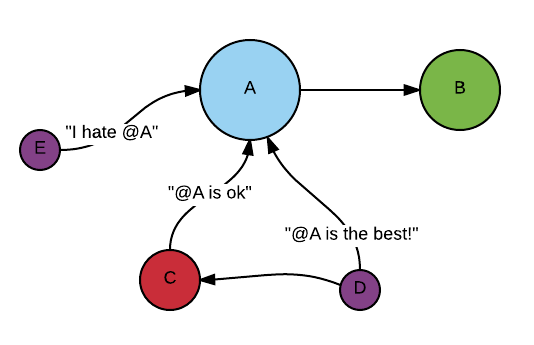
\includegraphics[width=3.5in,natwidth=534,natheight=345]{images/PageRank.png}
\caption{PageRank applied to the Twitter database. Every user is a node, while every mention in tweets is an edge. The size of the node is its relative rank among others.}
\label{fig:pagerank}
\end{figure}



Although the original PageRank algorithm was modeled with focus on the World
Wide Web, its method could be applied to any problem which can be modelled as a
graph. Specifically for Twitter, one could see each \emph{user} of the platform
as a node and every \emph{mention} in the tweets of a user to another as a link.
In the same way that web pages with high number of inlinks have a higher rank,
users that are mentioned frequently will be considered more relevant for our
recommendation engine, this process can be more clearly seen in Figure
\ref{fig:pagerank}. Note that we actually do not analyse the content of the
tweet, so tweets with positive or negative sentiment will have the same
importance for ranking, one could think of it being a "any publicity is good
publicity" kind of model.

% In our case, the probability of following a user (outlink) is proportional to
% the number of followers the corresponding user has.
The original PageRank algorithm considered following an outlink with equal
probability among all the possible links. That is reasonable with the
unstructured meta information available in the Web today, but is intuitive to
reason that, with more information about these users, different probabilities
could be applied to each one of them, depending on the task that we have at
hand. For a user recommender engine, our approach used the \emph{number of
followers} as a good measure of importance. That is, users with high number of
followers will be jumped to with higher probability in the random walk, so their
score will be naturally higher. Our engine implemented both methods for
evaluation, and the results are reported in the Experiments section.

\subsubsection{PageRank Monte Carlo}

The standard implementation of the PageRank computation is done via a method called power iteration. This method, although popular and still used today
by Google, has its drawbacks mainly regarding the speed of convergence, several
passes may be needed until the desired precision is obtained. In our approach we
explored a relatively new method, which utilize \emph{Monte Carlo algorithms} as proposed by Avrachenkov et al.
\cite{prmc} to
estimate the score of the nodes of the graph.

Of the several different algorithms proposed, our engine implements the
\emph{Monte Carlo complete path}, which is detailed in the Algorithm
\ref{alg:prmc}. For every user in the Twitter database, we start a random walk
beginning in that user and ending when the user is bored of following mentions.
We keep track of the total steps of all random walks and how many times each
user was visited. A new user is selected to be followed in the walk from all the
users the user mentions, which can be done by applying equal probabilities to
each one of them or with increased chance for higher number of followers. If a
user does not mention anyone, we consider it a \emph{sink} and jump to any other
user in the database with the same method. After every user has been at the
beginning of the random walk for a set number of walks, we calculate the user
rank by dividing the number of times each user was visited over all random walks
with the total steps taken.

\begin{algorithm}[H]
\caption{PageRank Monte Carlo, complete path}\label{alg:prmc}
\begin{algorithmic}
\Procedure{PageRank}{}
\ForAll{walks}
\ForAll{user in users}
	\State $\textit{username} \gets \textit{user['username']}$
    \State $\textit{bored} \gets \textit{False}$
    \While{$\neg bored$}
		\State $\textit{totalSteps} \gets $\textit{totalSteps} + 1
        \State $\textit{userSteps['username']} \gets \textit{userSteps['username']} + 1$
        \State $\textit{mentions} \gets \textit{getUserMentions(username)}$
     	\If{$mentions \in \emptyset$ }
                \State $\textit{username} \gets \textit{getRandomUser(users)}$
        \Else
     		\State $\textit{username} \gets \textit{getRandomUser(mentions)}$
        \EndIf
        \State $\textit{bored} \gets \textit{isUserBored()}$
    \EndWhile
\EndFor
\EndFor

\ForAll{user in users}
	\State $\textit{username} \gets \textit{user['username']}$
	\State $\textit{ranks['username']} \gets userSteps['username'] \div totalSteps $
\EndFor

\State \Return {$ranks$}

\EndProcedure
\end{algorithmic}
\end{algorithm}


\subsection{tf-idf}



\subsection{Graphical user interface}
